\documentclass[12pt,a4paper]{article}
\usepackage[german]{babel}
\usepackage{mycv}
\usepackage{array}
\usepackage{multicol}
\usepackage{longtable}
\usepackage{xcolor}
\usepackage[utf8]{inputenc}
\usepackage[pdfborder={0 0 0}]{hyperref} 
\usepackage[T1]{fontenc}
\usepackage[left=2.5cm,right=2.5cm,top=2.5cm,bottom=2.5cm]{geometry}
\usepackage{parskip}


\def\platz{Familienstandxxxxxxxxxxxx}
\begin{document}
\pagestyle{empty}

{\small
\begin{center}
Dr. Robert Haas, 
Brudermühlstra\ss{}e 34 a, D-81371 M\"unchen\\
Telefon: 0176 8018 1926, Email: Haasrobert@gmx.net
\end{center}
\vskip1em%
\hrule
\vskip4em%
}


\begin{flushright}
München, \today
\end{flushright}
\vskip0.8em
\noindent
%%% Adressat 1 Begin
Berufliche Oberschule Fürstenfeldbruck\\
Münchner Str. 67\\
82256 Fürstenfeldbruck
%%% Adressat 1 End
\vskip2em
\noindent
\textbf{Bewerbung als Lehrkraft an der Fach- und Berufsoberschule} \\
%
\vskip1.8em%
\noindent
Sehr geehrte Damen und Herren der Schulleitung,
\vskip0.5em%
\noindent
mit großem Interesse bewerbe ich mich als Lehrkraft für die Fächer Mathematik, Physik und Informatik an Ihrer Fach- und Berufsoberschule. Im erstgenannten Fach Mathematik habe ich 2002 mein Diplomstudiengang an der TU Chemnitz abgeschlossen. Anschließend habe 2007 an der Universität Regensburg promoviert. Diese fundierte Ausbildung möchte ich nun gerne im schulischen Kontext einbringen. 
\vskip0.5em%
\noindent
Während meiner wissenschaftlichen Tätigkeit habe ich gelernt, komplexe Inhalte strukturiert und verständlich zu vermitteln. Der Unterricht an einer weiterführenden Schule bietet mir die Möglich- keit, junge Menschen für mathematisch-naturwissenschaftliche Themen zu begeistern und sie auf ihrem Bildungsweg zu begleiten. Auch ohne bisherige Lehramtsausbildung bin ich überzeugt, dass ich durch meine Fachkompetenz, analytisches Denken und pädagogisches Interesse eine wertvolle Ergänzung für Ihr Kollegium darstellen kann.
\vskip0.5em%
\noindent
Ich strebe einen Quereinstieg gerne für das kommende Schuljahr oder das Schuljahr 2026/2027 an und bin bereit, die dafür erforderlichen Qualifizierungsmaßnahmen zu absolvieren. Über die Möglichkeit eines persönlichen Gesprächs würde ich mich sehr freuen.
%
\vskip1.3em
\noindent
Mit freundlichen Grüßen,
\vskip0.5em%
\noindent
\begin{tabular}{l}
\scalebox{0.6}{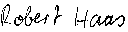
\includegraphics{signature}}
\end{tabular}\\
\noindent
Robert Haas
\vskip0.3em% 
\noindent


\newpage

{\small
\begin{center}
Dr. Robert Haas, 
Brudermühlstra\ss{}e 34 a, D-81371 M\"unchen\\
Telefon: 0176 8018 1926, Email: Haasrobert@gmx.net
\end{center}
\vskip1em%
\hrule
\vskip4em%
}

\vskip10em%
\centerline{
 \begin{tabular}{c}
 \scalebox{0.25}{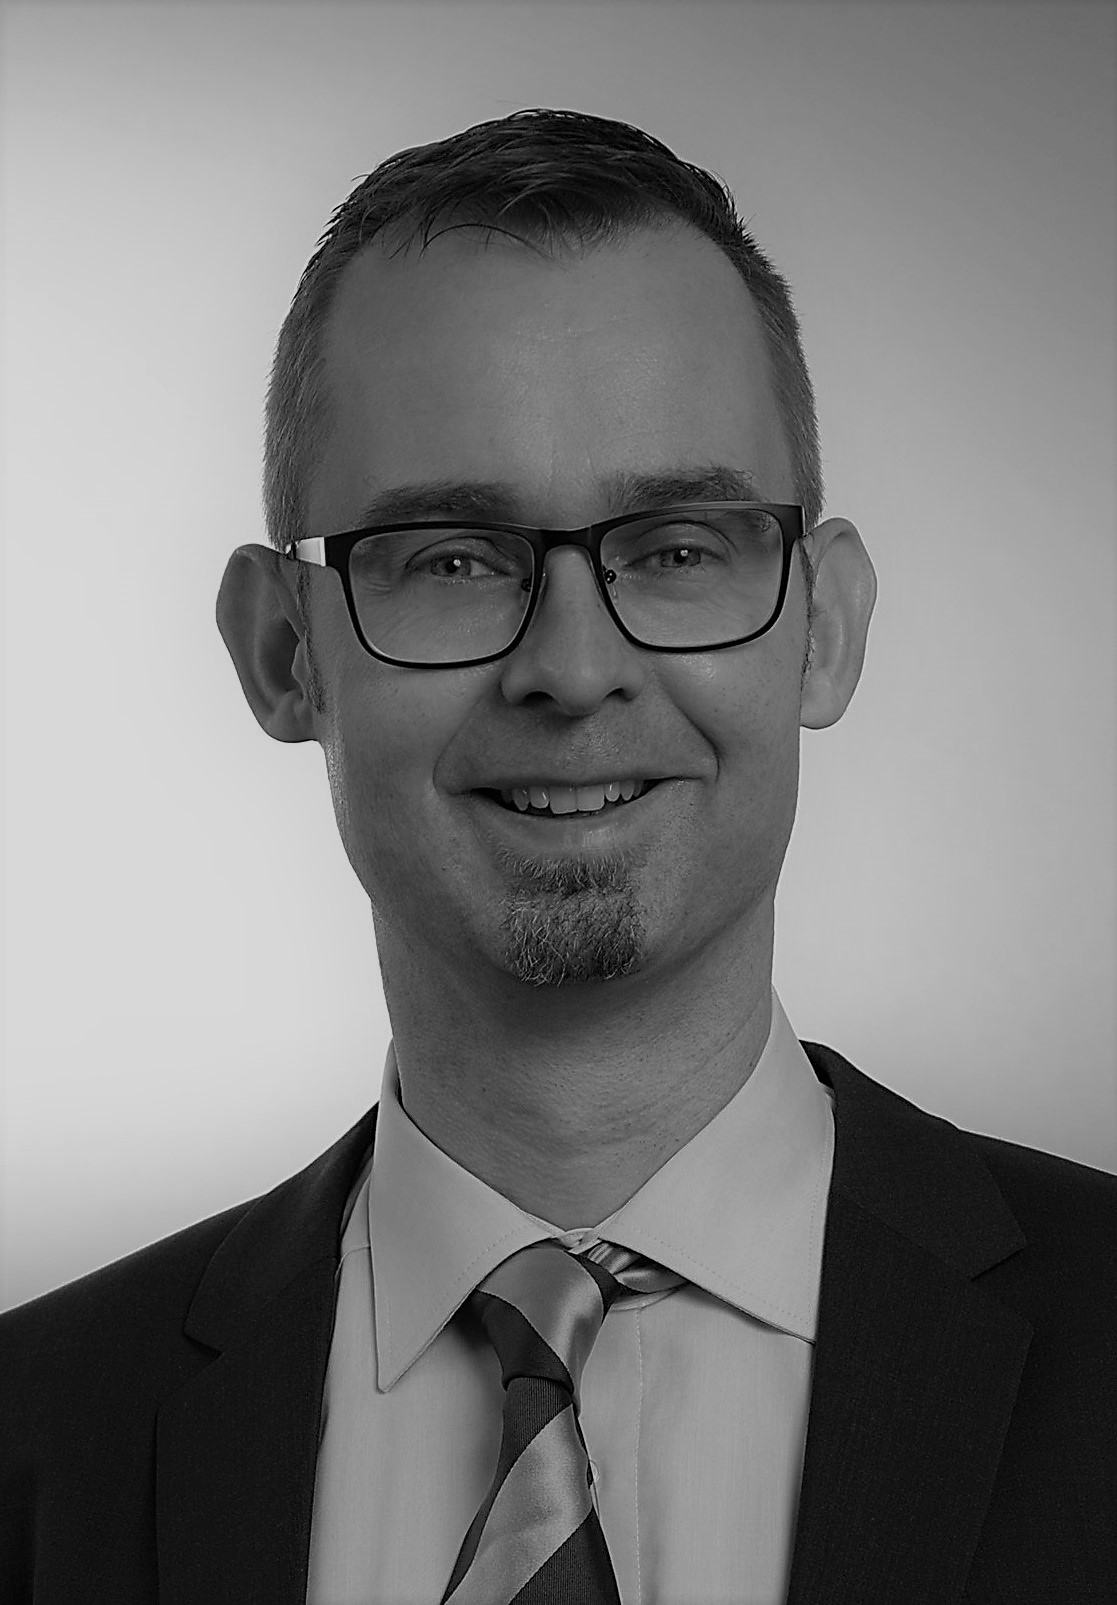
\includegraphics{Robert_Haas_2020_mc}}
 \end{tabular}
}
\vskip10em%
\begin{center}{\Huge Bewerbungsunterlagen f\"ur\vskip0.5em%
\noindent
%%% Adressat 2 Begin
Berufliche Oberschule Fürstenfeldbruck
%%% Adressat 2 End
}
\end{center}

\newpage

{\small
\begin{center}
Dr. Robert Haas, 
Brudermühlstra\ss{}e 34 a, D-81371 M\"unchen\\
Telefon: 0176 8018 1926, Email: Haasrobert@gmx.net
\end{center}
\vskip1em%
\hrule
\vskip4em%
}

\section*{Lebenslauf}
\subsection*{Persönliche Daten}
\begin{tabbing}
\platz \= ledig \= \kill
Geburtsdatum: \> 06.08.1975 \\
Geburtsort: \> Saalfeld \\
Familienstand: \>  ledig \\
Profil in LinkedIn: \> \href{https://www.linkedin.com/in/robert-haas-saalfeld/}{\color{blue} linkedin.com/in/robert-haas-saalfeld/}\\
Github-Account: \> \href{https://github.com/Haasrobertgmxnet}{\color{blue} github.com/Haasrobertgmxnet}\\
\end{tabbing}
%
\subsection*{Kenntnisse in Mathematik}
Variationsrechnung, Gewöhnliche und partielle Differentialgleichungen, mathematische Modellierung, mathematische Physik, Analysis, Lineare Algebra, numerische Verfahren für Differentialgleichungen
%
\subsection*{Kenntnisse im maschinellen Lernen}
Physics-Informed Neural Networks (PINNs), Multilayer Perceptron, Naive-Bayes-Classifier, Support-Vector-Machines, OpenNN, MLPack, PyTorch, Tensorflow/Keras
%
\subsection*{EDV-Kenntnisse}
C++, Python, R, R Shiny-App, Matlab, C\#, WPF, Xamarin/Prism, MS Visual Studio, Visual Studio Code, Git, Doxygen, Jabref
%
\subsection*{Kenntnisse in Statistik und Inferenzstatistik}
Varianzanalyse, Fallzahlplanung, Trennschärfe, Effektgröße, Konfidenzintervalle, Kruskal-Wallis-Test, Scheirer-Ray-Hare-Test, Aligned-Rank-Transform, Cohen's Power Tables
%

\subsection*{Fremdsprachen}
Englisch, Spanisch (sehr gut), Französisch (Grundkenntnisse)\\

\newpage
\pagestyle{empty}
{\small
\begin{center}
Dr. Robert Haas, 
Brudermühlstra\ss{}e 34 a, D-81371 M\"unchen\\
Telefon: 0176 8018 1926, Email: Haasrobert@gmx.net
\end{center}
\vskip1em%
\hrule
\vskip4em%
}

%\vskip0.01em%
\subsection*{Anstellungen, 15.02.2021 bis heute}
\begin{tabular}{l|l}
01.01.2025 -- 17.04.2025 & {\bf Open Mind Technologies AG, Wessling}\\
& Softwareentwicklung im Bereich Geometrie/CAM in C++\\
%
14.09.2022 -- 31.12.2024 & {\bf MCA Engineering GmbH, München}\\
& Arbeitnehmerüberlassung bei MTU Aero Engines AG München\\
& Entwicklung von Abnahme- und Akzeptanztests, Automatisierung\\
%
01.10.2021 -- 15.08.2022 & {\bf Leevi Health GmbH (jetzt Lilio Gmbh), Garching}\\
& Spezialalgorithmen und Machine-Learning-Verfahren zur \\
& Verarbeitung physiologischer Zeitreihen\\
%
15.02.2021 -- 31.08.2021 & {\bf Biomed GmbH, Oberschleißheim}\\
& Vergleich von Chargen und Kalibratoren \\
& mit statistischen Methodenvergleichen\\
& Tool zur statistischen Ermittlung und Analyse\\
& von Kennwerten in reguliertem Umfeld\\
%
\end{tabular}
%
\subsection*{Projekte als Selbständiger, 01.03.2018 bis 14.02.2021}
%
\begin{tabular}{l|l}
01.12.2020 -- 14.02.2021 & {\bf Biomed GmbH, Oberschleißheim}\\
& Statistische Auswertung der beschleunigten Haltbarkeitsprüfung\\
& von In-vitro-Diagnostika\\
%\\
09.12.2019 -- 14.12.2019 & {\bf Statistik-Projekt, München}\\
& Beratung zur statistischen Auswertung einer Umfrage,\\
& Literaturrecherche und Reliabilitätsschätzung in SPSS\\
%\\
20.03.2019 -- 24.10.2019 & {\bf Inchron GmbH, Potsdam}\\
& SW-Applikation zur Simulation von Embedded Systemen\\
& \begin{tabular}[t]{l}
{\em Eingesetzte Technologien:} C++- Desktop-Entwicklung (Linux), \\
verschiedene C++-Bibliotheken, Jira, Entwicklung nach Scrum\\
%\\
\end{tabular}\\
15.06.2018 -- 15.12.2018 & {\bf Rathgeber GmbH \& Co. KG, Oberhaching}\\
&  Entwicklung einer Datenbank-Anwendung \\
& \begin{tabular}[t]{l}
{\em Zweck:} C\#.NET-Desktop-Applikation für lesenden Zugriff\\
auf einen Microsoft-SQL-Server, Excel-Export\\
{\em Eingesetzte Technologien:} WPF/MVVM, Entity Framework,\\
Dependency Injection, Prism, Open XML SDK\\
%\\
\end{tabular}\\
%
01.01.2016 -- 30.06.2018 & {\bf Entwicklung einer eigenen technischen Software in C++} \\
%& Vorbereitung der beruflichen Selbständigkeit \\
& \begin{tabular}[t]{l}
{\em Zweck:} Modulare Programmbibliothek zur thermischen\\
 Berechnung von Wärmeübertragern %\href{http://engineering.roberthaas.net/calor-online-waermetauscherberechnung-leicht-gemacht}{\color{blue}Weitere Informationen}
\\
{\em Methoden:} Berechnungsverfahren aus VDI Wärmeatlas, \\
Objektorientierter Entwurf in C++ 11/C++ 14,\\
Zielplattformen Windows und Linux, CoolProp für Fluiddaten\\
\end{tabular}\\
%
\end{tabular}
%
\newpage
\pagestyle{empty}
{\small
\begin{center}
Dr. Robert Haas, 
Brudermühlstra\ss{}e 34 a, D-81371 M\"unchen\\
Telefon: 0176 8018 1926, Email: Haasrobert@gmx.net
\end{center}
\vskip1em%
\hrule
\vskip4em%
}

\subsection*{Berufsweg}
\vskip0.7em%
\begin{tabular}{l|l}
01.06.2012 -- 31.08.2017 & Angestellt bei {\bf EagleBurgmann Germany, Wolfratshausen} (2)\\
\\
01.12.2009 -- 31.05.2012 & Angestellt bei {\bf Ferchau Engineering, Rosenheim} (1)\\
& \begin{tabular}[t]{l}
Zunächst über (1) bei EagleBurgmann Germany eingesetzt,\\
danach bei (2) direkt angestellt. In beiden Fällen wurden\\
folgende Projekte bearbeitet:\\
{\em Entwicklung einer neuen Software zur Berechnung}\\
{\em technischer Daten von Dichtungssystemen:}\\
Modular aufgebauter Berechnungskern in Maple-Worksheets\\
Programmierung Algorithmen\\
Eigene Toolchain zur Generierung einer Library\\
Recherche, Analyse und Aufbereitung von Daten\\
Entwicklung von Tools in Matlab, VBA/Excel und AutoIt\\
Test und Dokumentation\\
Verwendung von Software für Wärmeübertrager und Fluiddaten\\
Unterstützung der GUI-Entwicklung\\
{\em Erweiterung eines vorhandenen Software-Tools}\\ 
{\em zur Auslegung von Dichtungssystemen:}\\
Anbindung moderner und effizienter Auswertungsverfahren\\
an vorhandenes Excel-Tool\\
Kommunikation zwischen Excel und der Software Optislang,\\
Entwicklung in C\#\\
Recherchen zu neuronalen Netzen und Optimierungsverfahren\\
\end{tabular}\\
\\
%
01.05.2007 -- 30.11.2009 & Angestellt bei {\bf Busch Vakuumpumpen und Systeme, Maulburg}\\
& \begin{tabular}[t]{l}
Auslegung zweiwelliger Verdrängerpumpen\\
Entwicklung von Auslegungsprogrammen\\
Differentialgeometrische Beschreibung neuer Rotorgeometrien\\
Konstruktion von Verzahnungsgeometrien\\
Rotordynamik und Auswuchtung\\
Thermodynamische Analysen, FEM\\
Patentwesen\\
\end{tabular}\\
%
\end{tabular}
%
\newpage
\pagestyle{empty}
{\small
\begin{center}
Dr. Robert Haas, 
Brudermühlstra\ss{}e 34 a, D-81371 M\"unchen\\
Telefon: 0176 8018 1926, Email: Haasrobert@gmx.net
\end{center}
\vskip1em%
\hrule
\vskip4em%
}

\subsection*{Berufsweg}
\vskip0.7em%
\begin{tabular}{l|l}
01.12.2006 -- 30.04.2007 & Fertigstellung und Abschluss Promotion\\
\\
%
16.05.2002 -- 30.11.2006 & {\bf Universität Regensburg}\\
& \begin{tabular}[t]{l}
Wissenschaftlicher Mitarbeiter am Lehrstuhl Prof. Garcke\\
DFG-Schwerpunktprogramm \glqq Phasenumwandlungen in\\
mehrkomponentigen Schmelzen\grqq\\
Entwicklung und Analyse mathematischer Modelle\\
Thermodynamik, Strömungsmechanik und\\
Materialwissenschaften\\
\end{tabular}\\
\\
%
01.04.2002 -- 15.05.2002 & Arbeitssuchend, Mithilfe in der Lutherkirche Chemnitz\\
\\
%
01.07.2001 -- 31.03.2002 & Softwareentwickler in Teilzeit, Informatik-DV, Crimmitschau\\
%
\end{tabular}
%
\subsection*{Schul- und Berufsausbildung}
\vskip0.7em%
\begin{tabular}{l|ll}
01.10.1995 -- 28.02.2002 & \multicolumn{2}{l}{Studium Mathematik an der TU Chemnitz, Diplom}\\
01.07.1994 -- 30.06.1995 & \multicolumn{2}{l}{Wehrdienst bei der Bundeswehr}\\
01.09.1990 -- 30.06.1994 & \multicolumn{2}{l}{Diesterweg-Gymnasium Plauen, Abitur}\\
01.09.1982 -- 30.08.1990 & \multicolumn{2}{l}{Schulen in Saalfeld und Plauen}\\
\end{tabular}
\vskip3.5em%
%\vskip1em%
%
\vskip2.5em%
\noindent
München, \today\\
\vskip0.2em%
\noindent
 \begin{tabular}{l}
 \scalebox{0.7}{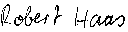
\includegraphics{signature}}
 \end{tabular}
\\
\noindent
 Robert Haas
 \newpage
 %
\pagestyle{empty}
{\small
\begin{center}
Dr. Robert Haas, 
Brudermühlstra\ss{}e 34 a, D-81371 M\"unchen\\
Telefon: 0176 8018 1926, Email: Haasrobert@gmx.net
\end{center}
\vskip1em%
\hrule
\vskip4em%
}

\section*{Lehrt\"atigkeit}
\vskip2em%
\begin{tabbing}
\platz \= \kill
Vorlesung \glqq{}Mathematik 2 für Wirtschaftsingenieure\grqq{} an der Hochschule München \\
\>Sommersemester 2024 \\
\\
Vorlesung \glqq{}Darstellende Geometrie\grqq{} an der Hochschule München \\
\>Sommersemester 2014 \\
\>Wintersemester 2013/14 \\
\\
Seminar \glqq{}Elliptische Differentialgleichungen\grqq{}, 2 SWS, an der Universität Regensburg\\
\\
Übung zur Vorlesung \glqq{}Numerische Mathematik II\grqq{}, 2 SWS, an der Universität Regensburg\\
\\ 
Betreuung von Diplomarbeiten und Abschlussarbeiten, an der Universität Regensburg\\
\\
Nachhilfeunterricht (Einzelunterricht) in Mathematik und Physik, freiberuflich \\
\end{tabbing}
\vskip2em%
\noindent
\end{document}
